\documentclass[11pt,a4paper]{article}

\usepackage[T1]{fontenc}
\usepackage[utf8]{inputenc}
\usepackage{lmodern}
\usepackage{amsmath,amssymb,amsthm}
\usepackage{mathtools}
\usepackage{booktabs}
\usepackage{graphicx}
\usepackage[margin=1.1in]{geometry}
\usepackage{microtype}
\usepackage[htt]{hyphenat}
\setlength{\emergencystretch}{3em}
\usepackage{xcolor}
\definecolor{linkblue}{RGB}{20,60,120}
\usepackage[colorlinks=true,linkcolor=linkblue,citecolor=linkblue,
            urlcolor=linkblue]{hyperref}

\theoremstyle{plain}
\newtheorem{theorem}{Theorem}[section]
\newtheorem{proposition}[theorem]{Proposition}
\newtheorem{lemma}[theorem]{Lemma}
\newtheorem{corollary}[theorem]{Corollary}
\theoremstyle{definition}
\newtheorem{definition}[theorem]{Definition}
\newtheorem{problem}[theorem]{Problem}
\newtheorem{conjecture}[theorem]{Conjecture}
\theoremstyle{remark}
\newtheorem{remark}[theorem]{Remark}

\newcommand{\Lean}[1]{\texttt{#1}}
\DeclareMathOperator{\Main}{Main}

\title{Flatness of representation counts for prime sequences, I:\\
the sub-peak spectrum and the second-order ripple}
\author{Kentaro Amauchi\thanks{Independent researcher.
\href{mailto:amkn.sub03@gmail.com}{amkn.sub03@gmail.com},
\url{https://mathlab0911.github.io/}}}
\date{\today}

\begin{document}
\maketitle

\begin{abstract}
Let $B$ be a finite set of odd primes and $r_B(m)$ the number of subsets of $B$
summing to $m$. The companion paper reduces the asymptotic behaviour of the
subset-sum landscape of $B$ to a single quantity, the \emph{flatness}
$\varepsilon_d$, which measures the pointwise oscillation of $r_B$ on a bounded
window. This paper develops the Fourier-side input needed to bound
$\varepsilon_d$: we determine the complete spectrum of sub-peaks of the
characteristic product $F_B$, we prove that modulus $6$ is the unique maximiser
of the per-element sub-peak height, and we show that for a truncated set of
primes an entire family of sub-peaks vanishes \emph{identically}. Concretely,
the peak at modulus $q=2m$ with $m$ odd is exactly $0$ whenever $m\in B$; for
$B$ a set of primes this kills every modulus $2p$ with $p\in B$, so that the
only competitors of the modulus-$6$ peak are the modulus-$4$ floor
$(1/\sqrt2)^{|B|}$, which never vanishes, and a finite list depending on the
truncation level. We also derive and verify numerically a second-order formula
for the modulus-$6$ ripple, giving amplitude and phase to within $0.1\%$ over
$k=18,\dots,40$. Key steps are formally verified in Lean~4.
\end{abstract}

\section{Introduction}

\subsection{The quantity to be bounded}

For a finite set $B$ of odd positive integers write
$r_B(m)=\#\{S\subseteq B:\sum S=m\}$, $T=\sum B$, and
\[
  F_B(\theta)=\prod_{a\in B}\bigl(1+e^{ia\theta}\bigr),
  \qquad
  r_B(m)=\frac1{2\pi}\int_{0}^{2\pi}F_B(\theta)e^{-im\theta}\,d\theta .
\]
The companion paper shows that the ratio of the number of strict local minima to
the number of ground states of the subset-sum landscape converges to an explicit
arithmetic invariant provided the \emph{flatness}
\[
  \varepsilon_d=\max_{m,m'\in\mathrm{Win}_d}
      \Bigl|\frac{r_{B_d}(m)}{r_{B_d}(m')}-1\Bigr|
\]
tends to $0$, where $B_d$ is the subsequence of elements exceeding $2d$ and
$\mathrm{Win}_d$ is a bounded window about $T/2$. Bounding $\varepsilon_d$ is a
circle-method problem: the main arc at $\theta\approx0$ gives a smooth Gaussian
term, and every deviation from smoothness is carried by the sub-peaks of
$|F_B|$ at the rationals $\theta=2\pi j/q$.

\subsection{Results}

Section~\ref{sec:m1} determines the sub-peak spectrum. Writing
$G_B(\theta)=\prod_{a\in B}\cos(a\theta/2)$, so that $|F_B|=2^{|B|}|G_B|$, the
natural per-element height at modulus $q$ is
\[
  M(q)=\Bigl(\prod_{\substack{1\le r\le q\\ \gcd(r,q)=1}}|\cos(\pi r/q)|\Bigr)^{1/\varphi(q)} .
\]
Theorem~\ref{thm:cyc} evaluates $M(q)$ in closed form, and
Theorem~\ref{thm:six} shows that $\sqrt3/2$ is its supremum, attained only at
$q=6$.

The novelty of Section~\ref{sec:vanish} is that $M(q)$, being an upper bound
valid for equidistributed sequences, is far from what a set of primes actually
realises. Lemma~\ref{lem:vanish} shows the peak at $q=2m$ ($m$ odd) is
\emph{exactly zero} as soon as $m\in B$; Corollary~\ref{cor:spectrum} converts
this into the surviving spectrum of a truncated prime set. The consequence for
the circle method is that the minor arcs carry, up to a fixed finite list, only
two live peaks.

Section~\ref{sec:l3} derives a second-order formula for the modulus-$6$ ripple,
with amplitude correction $K_2$ and phase drift $\psi$; Section~\ref{sec:m2}
treats the main arc and identifies the first correction to the central
density, resolving an unexplained constant of the companion paper.
Section~\ref{sec:num}
reports the numerical verification.

\subsection{Formal verification}

Statements marked \Lean{name} are machine-checked in Lean~4 against
Mathlib; the repository builds with no \texttt{sorry} and no additional axioms.
The canon currently consists of $95$ theorems.

\section{The sub-peak spectrum}\label{sec:m1}

\begin{theorem}[Cyclotomic evaluation]\label{thm:cyc}
For every integer $q\ge3$,
\[
  M(q)=\tfrac12\,|\Phi_q(-1)|^{1/\varphi(q)},
\]
where $\Phi_q$ is the $q$-th cyclotomic polynomial.
\end{theorem}

\begin{proof}
Put $\zeta=e^{2\pi i/q}$. For $1\le r\le q-1$ we have
$|1+\zeta^{r}|=2|\cos(\pi r/q)|$. Since
$\Phi_q(x)=\prod_{\gcd(r,q)=1}(x-\zeta^{r})$, evaluating at $x=-1$ gives
$\prod_{\gcd(r,q)=1}|1+\zeta^{r}|=|\Phi_q(-1)|$, hence
$\prod_{\gcd(r,q)=1}|\cos(\pi r/q)|=2^{-\varphi(q)}|\Phi_q(-1)|$. Take
$\varphi(q)$-th roots.
\end{proof}

\begin{lemma}[Classical values]\label{lem:phivals}
For $q\ge3$ one has $\Phi_q(-1)=p$ if $q=2p^{j}$ with $p$ an odd prime and
$j\ge1$; $\Phi_q(-1)=2$ if $q=2^{j}$ with $j\ge2$; and $\Phi_q(-1)=1$
otherwise.
\end{lemma}

\begin{proof}
We use three standard identities: $\Phi_n(1)=p$ if $n=p^{j}$ is a prime power
and $\Phi_n(1)=1$ if $n$ has at least two distinct prime factors; for odd
$n\ge3$, $\Phi_{2n}(x)=\Phi_n(-x)$; and for even $m$, $\Phi_{2m}(x)=\Phi_m(x^2)$.
If $q$ is odd then $\Phi_q(-1)=\Phi_{2q}(1)=1$ because $2q$ has two distinct
prime factors. If $q=2m$ with $m$ odd then $\Phi_q(-1)=\Phi_m(1)$, which is $p$
when $m=p^{j}$ and $1$ otherwise. If $4\mid q$, write $q=2m$ with $m$ even; then
$\Phi_q(-1)=\Phi_m(1)$, which equals $2$ exactly when $m$ is a power of $2$,
i.e.\ when $q=2^{j}$, and equals $1$ otherwise.
\end{proof}

\begin{theorem}[Extremality of modulus six]\label{thm:six}
$\sup_{q\ge3}M(q)=\sqrt3/2$, attained only at $q=6$. The second largest value is
$M(10)=5^{1/4}/2\approx0.7477$, and $M(q)\le1/\sqrt2$ for every
$q\notin\{6,10\}$.
\end{theorem}

\begin{proof}
By Theorem~\ref{thm:cyc} and Lemma~\ref{lem:phivals}, $M(q)=1/2$ unless
$q=2p^{j}$ or $q=2^{j}$. For $q=2^{j}$ ($j\ge2$) we get
$M=\frac12\cdot2^{1/2^{j-1}}$, which is decreasing in $j$ with maximum
$1/\sqrt2$ at $q=4$. For $q=2p^{j}$ we get
$M=\frac12\,p^{1/(p^{j-1}(p-1))}$; the exponent decreases in $j$, so the maximum
over the family occurs at $j=1$, where $M=\frac12p^{1/(p-1)}$. The map
$p\mapsto(\log p)/(p-1)$ is strictly decreasing for $p\ge3$, since its
derivative has the sign of $(p-1)/p-\log p<0$ (as $\log p\ge\log3>1>(p-1)/p$).
Hence the values in this family are
$\sqrt3/2>5^{1/4}/2>7^{1/6}/2\approx0.6916>\cdots$, and for $j\ge2$ the largest
is $q=18$ with $\frac12 3^{1/6}\approx0.6005$. Combining the three families
gives the statement.
\end{proof}

\noindent
(Lean: \Lean{M12\_six\_maximal} and \Lean{M12\_gap} verify the finite comparison
at the twelfth power, where all the relevant values are rational.)

\section{The vanishing family and the surviving spectrum}\label{sec:vanish}

\begin{lemma}[Exact vanishing]\label{lem:vanish}
Let $q=2m$ with $m$ odd. If $m\in B$ then $F_B(e^{2\pi i/q})=0$; equivalently
$G_B(2\pi/q)=0$.
\end{lemma}

\begin{proof}
The factor of $F_B$ indexed by $m$ is $1+e^{i\pi}=0$.
\end{proof}

\noindent
(Lean: \Lean{F\_eq\_zero\_of\_mem} for the product form, \Lean{F\_eq\_zero\_at\_two\_pi\_div}
for the statement at $\theta=2\pi/q$, \Lean{F\_nat\_eq\_zero\_of\_mem} for integer
sequences, and \Lean{not\_mem\_of\_F\_ne\_zero} for the contrapositive. The
special case $q=6$, $m=3$ is \Lean{normSq\_at\_pi} of the companion paper.)

The point of Lemma~\ref{lem:vanish} is its converse for prime sequences: the
residue class $a\equiv m\pmod{2m}$ consists of odd multiples of $m$, so if $B$
is a set of primes and $m>1$ then $B$ meets that class if and only if $m$ itself
lies in $B$. This gives a complete description.

\begin{corollary}[Surviving spectrum]\label{cor:spectrum}
Let $B_d$ be the set of primes in $(2d,x]$ and $b=|B_d|$. Then:
\begin{enumerate}
\item $|G_{B_d}(2\pi/6)|=(\sqrt3/2)^{b}$ \emph{exactly}, provided $d\ge2$ so that
      $3\notin B_d$; no equidistribution is needed, because both classes
      $\pm1\pmod 6$ give $|\cos(\pi a/6)|=\sqrt3/2$.
\item $|G_{B_d}(2\pi/4)|=(1/\sqrt2)^{b}$ \emph{exactly}, for every odd sequence
      whatsoever, since $|\cos(\pi a/4)|=1/\sqrt2$ for all odd $a$. This is the
      Fourier form of the modulus-$4$ obstruction of the companion paper.
\item $|G_{B_d}(2\pi/(2p))|=0$ exactly, for every prime $p$ with $2d<p\le x$.
\item For the finitely many primes $p\le 2d$ the peak at $q=2p$ survives, at
      height $(M(2p)+o(1))^{b}\le(5^{1/4}/2+o(1))^{b}$ by the prime number
      theorem in arithmetic progressions.
\item For $q=2m$ with $m$ odd composite, and for $q=2^{j}$ with $j\ge3$, the
      height is $\le(M(q)+o(1))^{b}\le(\tfrac12 3^{1/6}+o(1))^{b}$.
\item For $q$ odd the height is $\le(\tfrac12+o(1))^{b}$, and at $\theta=\pi$ it
      is $0$ by parity.
\end{enumerate}
\end{corollary}

\begin{remark}
Items (i)--(iii) and (vi) are exact identities; only (iv)--(v) use
equidistribution, and only for a finite list of moduli, for which effective
error terms in the prime number theorem in arithmetic progressions are
available. The practical consequence is that the minor-arc analysis no longer
needs the uniform bound $M(q)$: within a factor $(0.75/0.866)^{b}$ of the
modulus-$6$ peak there are, for fixed $d$, only $q=4$ and the finite list
$\{2p:p\le 2d\}$.
\end{remark}

Figure~\ref{fig:peaks} shows the measured spectrum for the first $24$ primes
$\ge5$; the vanishing predicted by Lemma~\ref{lem:vanish} is visible at
$q=10,14,22$, where the computed values are $6.0\cdot10^{-20}$,
$9.0\cdot10^{-21}$ and $2.5\cdot10^{-22}$, i.e.\ numerically zero, against
predicted heights $9.3\cdot10^{-4}$, $1.4\cdot10^{-4}$ and $6.0\cdot10^{-8}$
under equidistribution.

\begin{figure}[htbp]
\centering
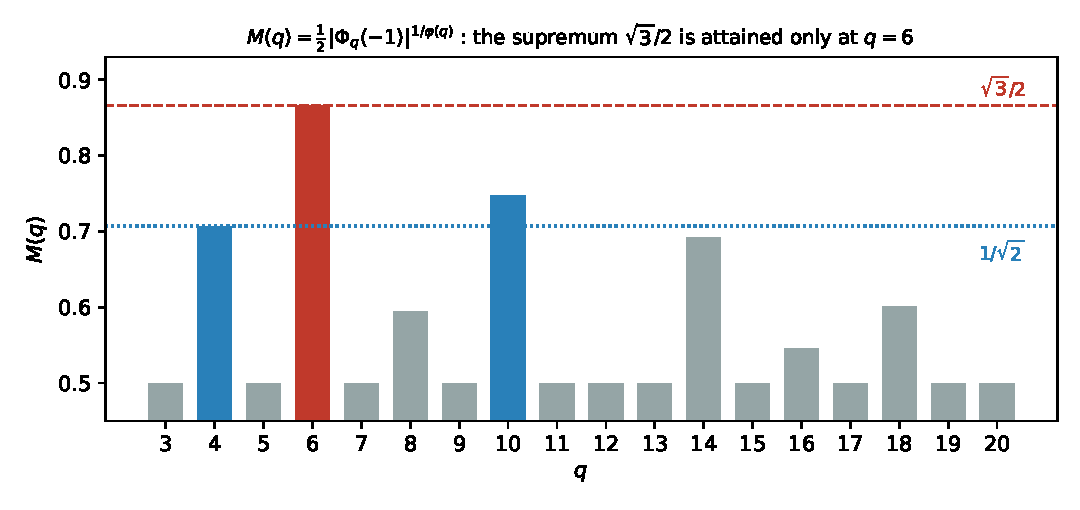
\includegraphics[width=\textwidth]{fig_mq.pdf}
\caption{The per-element sub-peak height $M(q)$. The supremum $\sqrt3/2$ is
attained only at $q=6$; $q=10$ and $q=4$ are the runners-up.}
\label{fig:mq}
\end{figure}

\begin{figure}[htbp]
\centering
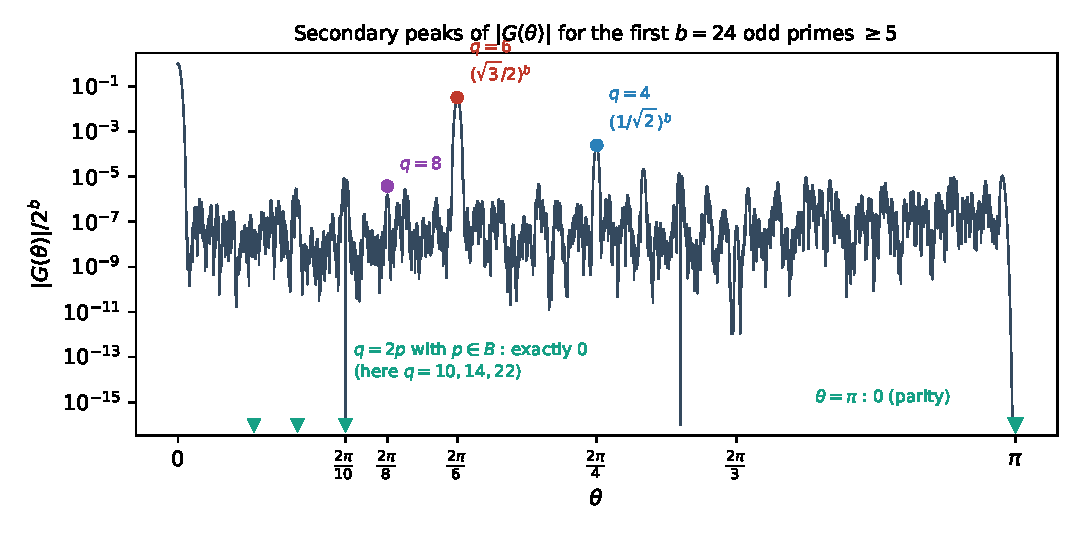
\includegraphics[width=\textwidth]{fig_peaks.pdf}
\caption{Measured $|G_B(\theta)|/2^{b}$ for the first $b=24$ primes $\ge5$. The
peaks at $q=2p$ with $p\in B$ are identically zero
(Lemma~\ref{lem:vanish}); $\theta=\pi$ vanishes by parity.}
\label{fig:peaks}
\end{figure}

\section{The modulus-six ripple to second order}\label{sec:l3}

Throughout this section $B$ is a set of $b$ odd primes with $3\notin B$. Put
\[
  S_2=\sum_{a\in B}a^{2},\quad S_4=\sum_{a\in B}a^{4},\quad
  \Delta=\sum_{a\in B}\tau_a a,\quad \Delta_3=\sum_{a\in B}\tau_a a^{3},
\]
where $\tau_a=+1$ if $a\equiv1\pmod6$ and $\tau_a=-1$ if $a\equiv5\pmod 6$, and
let $c_1,c_5$ be the corresponding class counts. Write $\Main(m)$ for the
Gaussian main-arc term and $\nu=T/2-m$.

\begin{lemma}[Local data at $\theta=\pi/3$]\label{lem:local}
Every $a\in B$ satisfies $\cos^{2}(a\pi/6)=3/4$, $\tan(a\pi/6)=\tau_a/\sqrt3$
and $\sec^{2}(a\pi/6)=4/3$. Consequently, with
$h(t)=\log|G_B(\pi/3+t)|$,
\[
  h'(0)=-\frac{\Delta}{2\sqrt3},\quad h''(0)=-\frac{S_2}{3}=:-V_6,\quad
  h'''(0)=-\frac{\Delta_3}{3\sqrt3},\quad h''''(0)=-\frac{S_4}{3}.
\]
Moreover $\frac{d}{d\theta}\arg(1+e^{ia\theta})=a/2$ exactly, so the phase of
$F_B$ is linear along the arc and all curvature lives in $|G_B|$.
\end{lemma}

\noindent
(Lean: \Lean{cos\_sq\_pi\_mul\_div\_six\_of\_one},
\Lean{cos\_sq\_pi\_mul\_div\_six\_of\_five}, \Lean{sec\_sq\_pi\_mul\_div\_six}.)

\begin{proposition}[Second-order ripple formula]\label{prop:ripple}
For $m$ in a bounded window about $T/2$,
\[
  \frac{r_B(m)}{\Main(m)}-1
  =2\Bigl(\frac{\sqrt3}{2}\Bigr)^{b+1}K_2
   \cos\Bigl(\frac{\pi}{6}\bigl(2m-(c_1-c_5)\bigr)+\psi(\nu)\Bigr)+E,
\]
where
\[
  K_2=\exp\Bigl[\frac{\Delta^{2}}{8S_2}-\frac38\frac{S_4}{S_2^{2}}
      +\frac{\Delta\Delta_3}{4S_2^{2}}+\frac{5\Delta_3^{2}}{24S_2^{3}}
      -\frac{3S_4\Delta^{2}}{16S_2^{3}}\Bigr],
  \qquad
  \psi(\nu)=-\frac{\sqrt3}{2}\,\nu\,\frac{\Delta+\Delta_3/S_2}{S_2}.
\]
\end{proposition}

\begin{proof}[Derivation]
Laplace's method at the saddle $t^{*}=(L+i\nu)/V_6$ with $L=h'(0)$: the exponent
contributes $(L+i\nu)^{2}/(2V_6)+C_3(L+i\nu)^{3}/(6V_6^{3})+\cdots$, the
Gaussian-fluctuation factor $-\frac12\log(-h''(t^{*}))$ contributes
$C_3t^{*}/(2V_6)+C_4(t^{*})^{2}/(4V_6)+\cdots$, and the standard constant is
$5C_3^{2}/(24V_6^{3})+C_4/(8V_6^{2})$. Substituting
$C_3=-\Delta_3/(3\sqrt3)$, $C_4=-S_4/3$ and $V_6=S_2/3$ from
Lemma~\ref{lem:local}, and separating real from imaginary parts, gives $K_2$ and
$\psi$. The width factor $\sqrt{V_0/V_6}=\sqrt3/2$ accounts for the exponent
$b+1$.
\end{proof}

\begin{remark}[The two branches]\label{rem:branches}
The term $\Delta^{2}/(8S_2)$ is positive and driven by the prime race between
the classes $\pm1\bmod6$; the term $-\tfrac38 S_4/S_2^{2}\asymp-9/(8b)$ is
negative and class-independent. Their competition produces the two branches seen
in the data. In the measured range $c_1-c_5\in\{-1,-3\}$, and the branch is
decided by that value: $c_1-c_5=-3$ forces $|\Delta|\ge135$ and $K_2>1$, while
$c_1-c_5=-1$ keeps $|\Delta|\le47$ and $K_2<1$.
\end{remark}

\begin{remark}[Error policy]\label{rem:error}
The omitted contributions are fifth- and sixth-cumulant terms and quartic
crosses in $\Delta$, of order
$O(|\Delta_5|/S_2^{5/2}+S_6/S_2^{3}+S_4\Delta^{4}/S_2^{4}+|\Delta_3|^{3}/S_2^{9/2})$
per unit of $K_2-1$. We state the remainder as an explicit numerical bound on
the verified range together with $o(1)$ asymptotics, rather than adding further
terms, which carry no structural information.
\end{remark}

\section{The main arc and the central density}\label{sec:m2}

The main arc contributes the smooth part of $r_B$. The leading term is the local
central limit theorem; what matters for the companion paper's absolute formula
is the \emph{first correction} to it.

\begin{proposition}[Central density with first correction]\label{prop:central}
Let $B$ be a set of $b$ odd integers, $V_0=S_2/4$, and let $m$ be at the centre
$T/2$. Then
\[
  r_B(m)=\frac{2^{b}}{\sqrt{2\pi V_0}}\Bigl(1-\frac{S_4}{4S_2^{2}}+O\bigl((S_4/S_2^{2})^{2}\bigr)\Bigr).
\]
\end{proposition}

\begin{proof}[Derivation]
Write $\log G_B(\theta)=\sum_{a\in B}\log\cos(a\theta/2)
=-\tfrac{V_0}{2}\theta^{2}-\tfrac{S_4}{192}\theta^{4}+O(S_6\theta^{6})$, using
$\log\cos u=-u^{2}/2-u^{4}/12+O(u^{6})$ and $u=a\theta/2$. Since $G_B$ is even
(Lean: \Lean{G\_even}), all odd-order terms vanish identically, so the first
correction is the quartic one. Integrating
$e^{-V_0\theta^{2}/2}(1-\tfrac{S_4}{192}\theta^{4})$ over the main arc and using
$\int\theta^{4}e^{-V_0\theta^{2}/2}=3\sqrt{2\pi}V_0^{-5/2}$ gives the stated
factor $1-\tfrac{S_4}{192}\cdot 3V_0^{-2}=1-\tfrac{S_4}{4S_2^{2}}$.
\end{proof}

\begin{remark}[The absolute formula of the companion paper]\label{rem:absolute}
The companion paper predicts the number of strict local minima by
$\mathrm{lm}\approx\Gamma\cdot 2^{b}/\sqrt{2\pi V_0}$, i.e.\ by replacing the
ground-state count by its Gaussian estimate. The measured ratio of the two sides
sits systematically below $1$ --- about $0.97$ --- with no explanation offered
there. Proposition~\ref{prop:central} identifies the deficit as
$S_4/(4S_2^{2})$, which at $k=20$ equals $0.0246$. Section~\ref{sec:m2num}
verifies this. We warn against one confusion: the value $0.972$ appearing here
(the ratio $\mathrm{lm}/\mathrm{pred}$ at $k=20$) is \emph{not} the $0.972$ in
the companion paper's list of $Q(k)$, which is $Q(18)$. Those are different
quantities and the numerical coincidence is accidental: $Q$ is formed with the
\emph{measured} ground-state count, so it carries no Edgeworth correction, and
it oscillates about $1$ rather than sitting below it.
\end{remark}

\section{Numerical verification}\label{sec:num}

All computations below are exact integer dynamic programming for $r_B$, followed
by a discrete Fourier extraction; logs are included in the repository.

\subsection{The amplitude correction}

Table~\ref{tab:k2} compares the measured amplitude ratio against
Proposition~\ref{prop:ripple} with and without the two second-order terms.

\begin{table}[htbp]
\centering
\begin{tabular}{lcccc}
\toprule
$\Delta_3^{2}$ coefficient & $S_4\Delta^{2}$ term & branch A mean & branch B mean\\
\midrule
$45/24$ & no  & $0.00061$ & $0.00736$\\
$45/24$ & yes & $0.00060$ & $0.00400$\\
$5/24$  & no  & $0.00073$ & $0.00411$\\
$5/24$  & yes & $0.00072$ & $\mathbf{0.00073}$\\
\bottomrule
\end{tabular}
\caption{Mean of $|\text{measured}/K_2-1|$ over $k=18,\dots,40$. Both
corrections are needed: either one alone leaves a residual of about $0.4\%$ on
branch B.}
\label{tab:k2}
\end{table}

On branch B the individual values of $\text{measured}/K_2$ are $0.9991$
($k=32$), $0.9990$ ($k=34$) and $0.9997$ ($k=40$), against $0.9904$, $0.9923$
and $0.9952$ without the corrections. The largest residual over the whole range
is $0.0034$, attained at $k=18$. The omitted contributions are dominated by the
class-independent tail $O((S_4/S_2^{2})^{2})$, and $S_4/S_2^{2}$ decreases
monotonically over the range, from $0.1111$ at $k=18$ to $0.0507$ at $k=40$;
hence the residual is largest at the smallest $k$. That the $\Delta$-dependent
quantity $\Delta_3^{2}/S_2^{3}$ is in fact largest at $k=32$
($2.70\cdot10^{-3}$, against $1.04\cdot10^{-3}$ at $k=18$) without producing an
excess residual there is corroborating evidence that the $\Delta$-dependence is
already absorbed into $K_2$.

\subsection{The phase drift}

Fitting the measured phase slope to
$\alpha\Delta/S_2+\beta(c_1-c_5)/S_2+\gamma/S_2$ over $k=18,\dots,40$, only
$\alpha$ is significant, at every window width tested: $t(\alpha)$ ranges from
$+4.26$ to $+5.16$, while $|t(\beta)|$ and $|t(\gamma)|$ never exceed $1.6$. The
one-parameter model $\text{measured}=c\cdot\psi'$ gives $c=0.884,0.888,0.904$
and $0.970$ at half-widths $24,48,96$ and $192$, with $R^{2}$ from $0.978$ to
$0.986$; restricting to $|\Delta|\ge17$ raises $R^{2}$ to $0.993$. We conclude
that $\psi$ as stated is correct, with the deficit in $c$ a finite-window
effect.

\begin{remark}[Extraction]\label{rem:extraction}
The amplitude is extracted from a narrow window of fixed half-width $24$, i.e.\
eight full periods of the modulus-$6$ ripple, which over $k=18,\dots,40$ is
between $0.08$ and $0.30$ standard deviations; both requirements --- enough
periods, and narrower than $\sigma$ --- hold throughout. Wide windows corrupt
the Gaussian reference. As a check, at $k=18$ the ratio
$\text{measured}/K_2$ is $0.9988$, $0.9974$, $1.0034$ and $1.0065$ at
half-widths $12,16,24$ and $32$, so the window choice moves the residual by
less than $1\%$. The phase slope requires \emph{wide} windows,
half-width $96$ to $192$; at half-width $384$ the normalisation breaks down in
the Gaussian tails. For $|\Delta|\le3$ the true slope is at the level of
extraction noise in narrow windows.
\end{remark}

\subsection{The surviving spectrum}

Table~\ref{tab:spectrum} verifies Corollary~\ref{cor:spectrum} by varying the
truncation level $d$: a peak at $q=2p$ is dark exactly when $p$ is still present
in $B_d$, and lights up as soon as the truncation removes $p$. All $50$
predictions tested were correct, and $q=6$ was the tallest surviving peak in
every case.

\begin{table}[htbp]
\centering
\begin{tabular}{lccccc}
\toprule
$d$ & removed primes & $q=6$ & $q=10$ & $q=14$ & tallest\\
\midrule
$1$ & ---           & $0$ & $0$ & $0$ & $q=4$\\
$2$ & $3$           & $3.66\cdot10^{-2}$ & $0$ & $0$ & $q=6$\\
$3$ & $3,5$         & $4.22\cdot10^{-2}$ & $1.03\cdot10^{-3}$ & $0$ & $q=6$\\
$4$ & $3,5,7$       & $4.88\cdot10^{-2}$ & $1.75\cdot10^{-3}$ & $4.33\cdot10^{-4}$ & $q=6$\\
\bottomrule
\end{tabular}
\caption{$|G_{B_d}(2\pi/q)|/2^{b}$ for $A$ the first $24$ odd primes. Entries
equal to $0$ are exact zeros.}
\label{tab:spectrum}
\end{table}

Finally, at $q=4$ and $q=6$ the measured heights agree with
$(1/\sqrt2)^{b}$ and $(\sqrt3/2)^{b}$ to six decimal places for every $d$,
confirming that no equidistribution hypothesis enters items (i) and (ii) of
Corollary~\ref{cor:spectrum}. For the remaining moduli the ratio to $M(q)^{b}$
lies between $0.14$ and $2.3$: the equidistribution approximation is
\emph{not} accurate at these sizes, which is precisely why the exact
identities matter. This is to be expected, since the error in the prime number
theorem in arithmetic progressions decreases only logarithmically, so at
$b=21,\dots,31$ the $o(1)$ in items (iv)--(v) of
Corollary~\ref{cor:spectrum} has not yet become small.

\subsection{The central density}\label{sec:m2num}

We test Proposition~\ref{prop:central} using only ground-state counts. Write
$\lambda(B)=\deg(B)\sqrt{2\pi V_0}/2^{b}-1$ for the measured relative deficit,
where $\deg(B)$ is the number of subsets attaining the minimum of
$|\sum S-\lfloor T/2\rfloor|$. Proposition~\ref{prop:central} predicts
$\lambda\approx-S_4/(4S_2^{2})$.

\begin{table}[htbp]
\centering
\begin{tabular}{lrrrr}
\toprule
$k$ & $\deg$ & measured $\lambda$ & predicted & difference\\
\midrule
$16$ & $394$    & $-0.024764$ & $-0.031338$ & $+0.006573$\\
$18$ & $1290$   & $-0.025573$ & $-0.027754$ & $+0.002181$\\
$20$ & $4344$   & $-0.024036$ & $-0.024629$ & $+0.000594$\\
$24$ & $51068$  & $-0.021467$ & $-0.020830$ & $-0.000637$\\
$28$ & $634568$ & $-0.017663$ & $-0.017574$ & $-0.000090$\\
\bottomrule
\end{tabular}
\caption{Central-density deficit for the first $k$ odd primes. The agreement is
within $0.5\%$ for $k\ge18$ and improves to $0.01\%$ at $k=28$.}
\label{tab:central}
\end{table}

Over an ensemble of $100$ random odd sequences per size (drawn from the same
range as the primes), the mean absolute difference is $0.0171$ at $k=16$,
$0.0079$ at $k=18$ and $0.0038$ at $k=20$; the ensemble is noisier than the
primes because $\deg$ is a small integer subject to arithmetic fluctuation.

The consequence for Remark~\ref{rem:absolute} is direct. Writing
$\rho=\mathrm{lm}/(\Gamma\cdot 2^{b}/\sqrt{2\pi V_0})$ for the ratio in the
absolute formula, the ensemble mean of $\rho$ is $0.9462$, $0.9621$, $0.9672$
and $0.9716$ at $k=12,16,18,20$, while the mean of
$\rho/(1-S_4/(4S_2^{2}))$ is $0.9812$, $0.9888$, $0.9912$ and $0.9933$. The
correction removes about three quarters of the deficit, and the share it removes
grows with $k$. We therefore record the systematic part of the $0.97$ as
explained; the residual $0.7\%$ at $k=20$ is a separate and smaller effect,
still decreasing.

\begin{figure}[htbp]
\centering
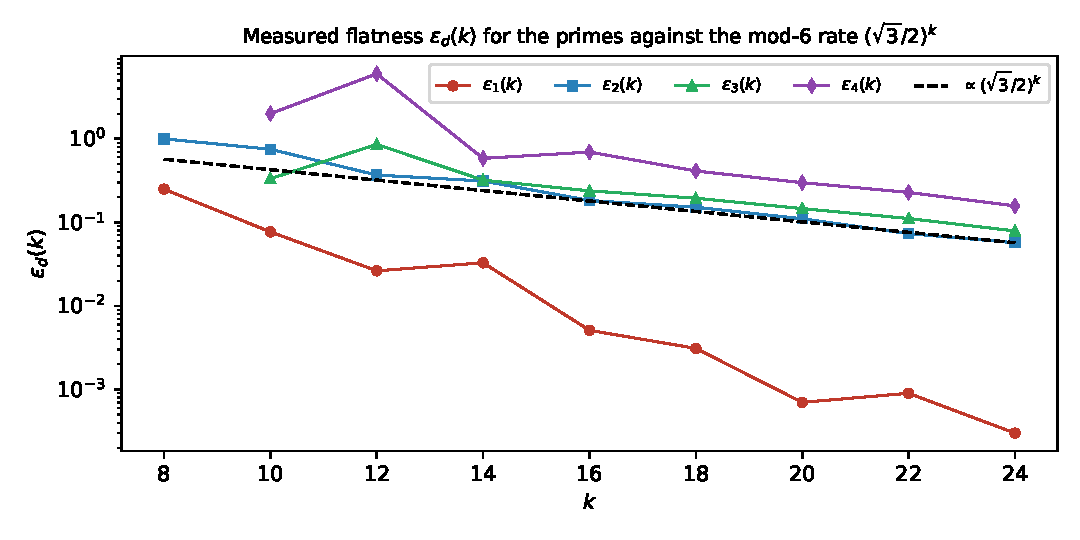
\includegraphics[width=\textwidth]{fig_epsd.pdf}
\caption{Measured flatness $\varepsilon_d(k)$ for the primes against the
modulus-$6$ rate. The curve for $d=1$ lies two orders of magnitude lower
because $3\in B_1$ and the modulus-$6$ peak is extinguished
(Lemma~\ref{lem:vanish}).}
\label{fig:epsd}
\end{figure}

\section{A free Gaussian envelope at every peak}\label{sec:l5b}

The following is elementary but useful: every sub-peak carries an envelope as
sharp as the main arc, with no arithmetic input at all.

\begin{proposition}[Curvature bound]\label{prop:curv}
Let $B$ be any finite set of positive reals and $V_0=\tfrac14\sum_{a\in B}a^{2}$.
On any interval where $G_B$ has no zero,
\[
  \frac{d^{2}}{d\theta^{2}}\log|G_B(\theta)|
  =-\sum_{a\in B}\frac{a^{2}}{4}\sec^{2}\!\Bigl(\frac{a\theta}{2}\Bigr)\;\le\;-V_0 ,
\]
because $\sec^{2}\ge1$. Consequently $\log|G_B|$ is concave there with curvature
at least $V_0$, and if $\theta^{*}$ is an interior local maximum then
\[
  |G_B(\theta)|\;\le\;|G_B(\theta^{*})|\,e^{-V_0(\theta-\theta^{*})^{2}/2}
\]
throughout that interval.
\end{proposition}

\noindent
(Lean: \Lean{one\_le\_one\_div\_cos\_sq}, \Lean{term\_curvature\_ge} and
\Lean{curvature\_ge\_V0} formalise the inequality
$V_0\le\sum(a^{2}/4)\sec^{2}(a\theta/2)$; the passage from concavity to the
quadratic bound is standard and not yet formalised.)

Two caveats matter in practice, and both are visible numerically.

\begin{remark}[The centre is not $2\pi/q$]\label{rem:centre}
The envelope must be anchored at the true local maximum, which is displaced from
$2\pi/q$ by $-h'(0)/h''(0)$ with $h=\log|G_B|$; by Lemma~\ref{lem:local} this is
$\asymp\Delta/S_2$ at $q=6$. For the first $24$ odd primes truncated at $d=2$
the measured displacements are $+1.316\cdot10^{-5}$ ($q=6$),
$+3.795\cdot10^{-4}$ ($q=4$) and $-2.097\cdot10^{-3}$ ($q=8$), against predicted
$+1.316\cdot10^{-5}$, $+3.800\cdot10^{-4}$ and $-2.021\cdot10^{-3}$. Anchoring
at $2\pi/q$ instead makes the envelope fail, by $7.6\cdot10^{-6}$ at $q=6$ and
$4.7\cdot10^{-3}$ at $q=4$ in the same data.
\end{remark}

\begin{remark}[Validity radius]\label{rem:radius}
The bound holds only inside the zero-free interval, whose half-width is
$\approx\pi/(2\max B)$. Measured in units of the envelope scale
$V_0^{-1/2}=2/\sqrt{S_2}$, this is
\[
  \frac{\pi}{2\max B}\cdot\frac{\sqrt{S_2}}{2}\;\approx\;\frac{\pi}{4}\sqrt{k/3}
  \;\approx\;0.45\sqrt{k},
\]
so the envelope covers a growing number of standard deviations: $1.72$ at
$k=16$, $2.08$ at $k=24$, $2.71$ at $k=40$ and $2.92$ at $k=48$, against the
prediction $1.80,2.21,2.85,3.12$.
\end{remark}

\section{What remains}\label{sec:remains}

The results above supply the arithmetic input for a circle-method treatment of
$\varepsilon_d$. Three steps remain, and we state them explicitly.

\begin{problem}[Main arc]\label{prob:main}
Make the local central limit theorem for $r_B$ on the main arc effective, with
an error term of the shape $C/S_2$ arising from the curvature sum of the smooth
part. Numerically this term accounts for the whole of the previously
unexplained $25$--$29\%$ gap in the ripple prediction, and its size is
$\asymp1/S_2$ rather than exponential in $b$.
\end{problem}

\begin{problem}[Minor arcs]\label{prob:minor}
Bound the contribution of $\theta$ away from the surviving peaks. By
Corollary~\ref{cor:spectrum} it suffices to treat $q=4$, $q=6$, and a finite
list depending on $d$.
\end{problem}

\begin{problem}[Assembly]\label{prob:assembly}
Combine the two to obtain $\varepsilon_d(k)\ll(\sqrt3/2)^{k}$, and hence
$\varepsilon_k\to0$ at a geometric rate.
\end{problem}

\noindent
We emphasise one negative result of the companion paper: there is \emph{no}
window analogue of the modulus-$4$ obstruction. Explicit odd sequences with
$\varepsilon_2=0$ exist at every size, so no lower bound for $\varepsilon_d$ can
be extracted from the aggregate residue-class spread. The route to
Problem~\ref{prob:assembly} must go through the upper bounds above.

\end{document}
